\setcounter{chapter}{11}
\chapter{Dipôle RC}


\section{Rappels}
\etiquette{Pour commencer}
	Travailler la page 424: carte mentale, réactiver ses connaissances et flash test
	
%	\begin{center}
%	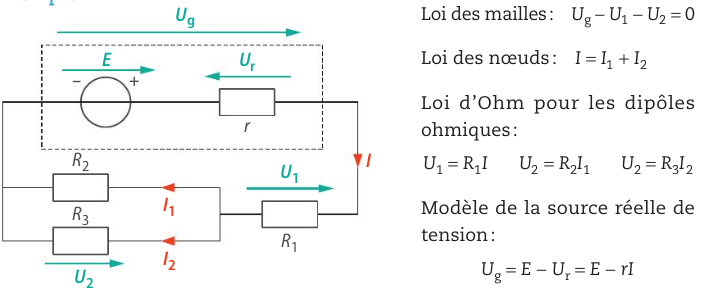
\includegraphics[scale=0.5]{figures/rc/rappels}
%	\end{center}

\section{Courant électrique: débit de charges}
\blocrouge{Définition}{\textbf{En régime permanent, indépendant du temps,} si pendant une durée $\Delta t$ une charge électrique Q traverse une section de conducteur, on définit l'intensité du courant :
\begin{center}
\trou{$I=\dfrac{Q}{\Delta t}$}
\end{center}
\textbf{En régime variable, dépendant du temps,} l'intensité i dépend du temps, on écrit i(t) ou simplement i. L'intensité du courant comme étant un débit de charges électriques. Cela correspond à la charge électrique qui traverserait une section de conducteur durant 1 seconde.  i se calcule en dérivant la fonction $q(t)$:
\begin{center}
\trou{$i(t)=\dfrac{dq}{dt}$}
\end{center}}

\etiquette{Application} Si à chaque seconde, la section d'un fil est traversée par une charge de 3 coulomb cela signifie que $$q(t)= 3\times t$$ on dit alors que l'intensité du courant qui traverse la section du fil vaut :$$i(t)= \trou{\dfrac{d(3t)}{dt	}=3\:A}$$

\section{Le condensateur}
	\subsection{De quoi est fait  un condensateur ?}
	
Un condensateur est composé de deux surfaces conductrices, placées face à face, les armatures. Elles sont séparées par un matériau isolant. \\
le symbole d'un condensateur est le suivant :\\
\begin{center}
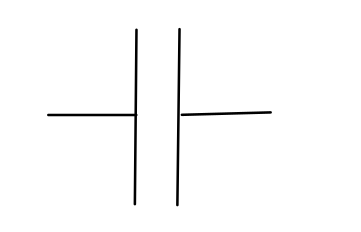
\includegraphics[scale=0.3]{figures/rc/condo}
\end{center} 

	\subsection{Phénomène de charge d'un condensateur}
	
Lorsqu'il est soumis à une tension électrique, le condensateur <<condense>> les charges positives d'une part et négatives d'autre part. Les charges s'accumulent sur \trou{les armatures}.\\
Les deux armatures d'un condensateur portent des charges électrique \trou{opposées}. On dit que le condensateur se \trou{charge}. Dans le même temps, une tension électrique apparaît entre les armatures. On la note \trou{$u_C$}.
\begin{center}
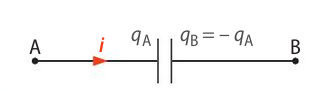
\includegraphics[scale=0.5]{figures/rc/condo2}
 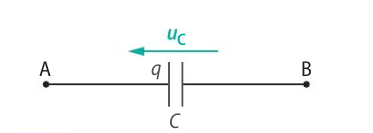
\includegraphics[scale=0.5]{figures/rc/uc}
\end{center}
 L'aptitude d'un condensateur à accumuler sur ses surfaces conductrices un grand nombre de charges électriques est appelée capacité. \\
  La capacité se note C et se mesure en \trou{farad (F)}\\



	\href{https://phet.colorado.edu/sims/html/capacitor-lab-basics/latest/capacitor-lab-basics_en.html}{Simulation condensateur}
	
	
	\subsection{Formules pour le condensateur}
		\begin{center}
					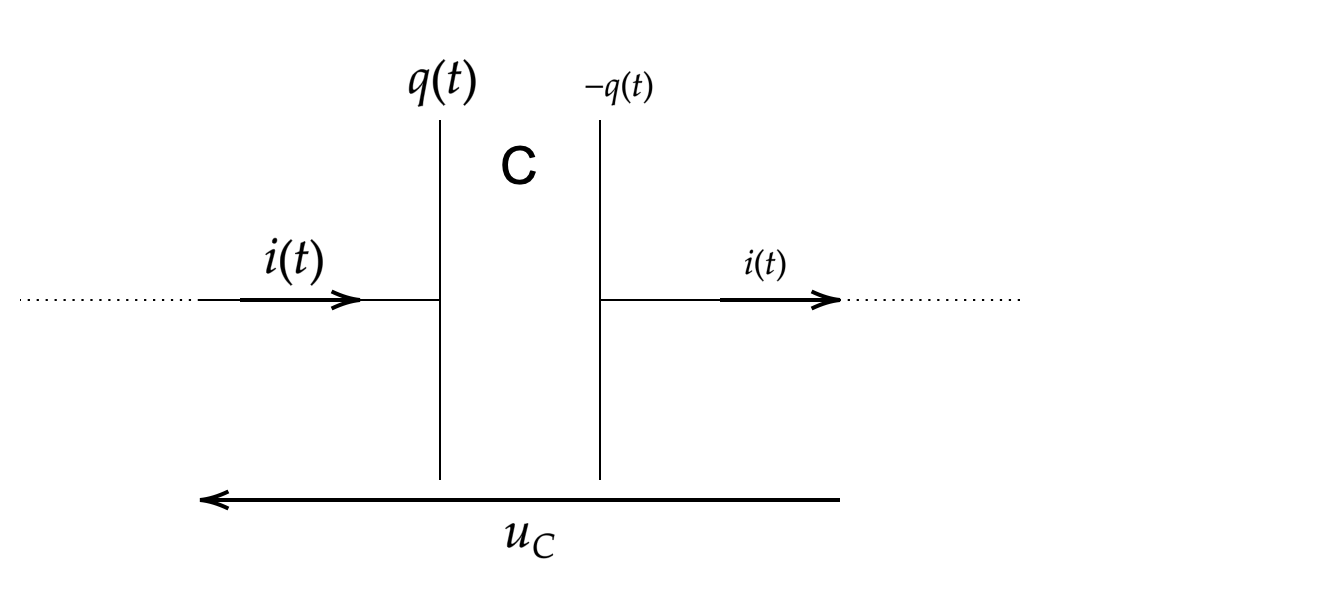
\includegraphics[scale=.18]{figures/rc/rc_resume}
		\end{center}
		\etiquetterouge{Relation Tension - Charge}
		$$\boxed{q=C\times u_C}$$
		$q$ en coulomb (C) ; C en Farad (F) et $u_C$ en volt (V)
			
	\etiquette{Comment la géométrie du condensateur modifie sa capacité ?}
	
	\begin{itemize}
		\item Si on augmente la surface des plaques alors \trou{la capacité du condensateur augmente.}
		\item Si on augmente la distance entre les plaques alors  \trou{la capacité du condensateur diminue.}
	\end{itemize}

	
			\etiquetterouge{Relation Courant - Tension} 
		
		On a vu que $$i(t)=\dfrac{dq}{dt}$$ en remplaçant $q$ par $C\times u_C$ on obtient $$i=\trou{\dfrac{d(C\times u_C)}{dt} }$$ Puisque $C$ est constant, on peut le "sortir" de l'opération de dérivation.

			$$\boxed{\trou{i=C.\dfrac{du_C}{dt}}}$$
	\subsection{Capteurs capacitifs}
Un capteur capacitif utilise les modifications de la capacité d'un condensateur. Ces modifications ont lieu lorsque la distance entre les armatures change, ou lorsque la nature de l'isolant change par exemple.\\
Exemples de capteurs capacitifs :
\begin{itemize}
\item \textbf{Capteur de \trou{ remplissage}} : Pour connaître le niveau de remplissage d'une cuve par exemple, on peut utiliser un capteur capacitif de remplissage. A mesure que le liquide remplit la cuve, l'isolant entre les armatures change (au départ, c'était de l'air, puis lorsque le niveau monte, cela devient le fluide). La capacité évolue donc en fonction de la hauteur de liquide qu'il contient.
\item \textbf{Capteur de \trou{position sur un écran tactile}} : Doc D et E p 429. La surface en verre d'un écran capacitif de smartphone comprend une grille de fils très fins électriquement chargée.\\
lorsqu'un doigt touche l'écran, des charges électriques sont transférées entre le doigt et l'écran, modifiant localement le champ électrique créé par ces fils. La détection de ces variations permet au téléphone de localiser la zone de contact doigt-écran.
\end{itemize}
\newpage

\section{Circuit RC série}  
	\subsection{Décharge d'un condensateur}

\blocgris{Situation}{
\begin{center}
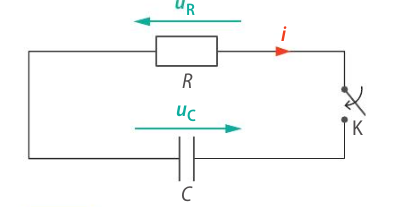
\includegraphics[scale=0.4]{figures/rc/decharge}
\end{center}

On dispose d'un condensateur initialement chargé: $\trou{u_c(t=0)= E}$ (tension E à ses bornes). Le condensateur est branché en série avec un conducteur ohmique de résistance R.\\ A l'instant $t=\SI{0}{\second}$, on ferme l'interrupteur. 
}


\etiquetterouge{Objectif} Trouver l'expression mathématique de la tension \trou{$u_c(t)$} aux bornes du condensateur pendant sa décharge.\\
\etiquette{Stratégie} 
\begin{enumerate}
	\item Appliquer la loi des mailles
	\item Utiliser les formules du condensateur pour écrire une équation différentielle en $u_c(t)$
	\item Résoudre l'équation différentielle en utilisant une condition initiale
\end{enumerate}

\etiquette{Etape 1: loi des mailles}
D'après la loi des mailles dans le circuit, on a :
\begin{center}
$0=\trou{u_c}+\trou{u_R}$ 
\end{center}
\etiquette{Etape 2: formules}
$$u_R=Ri=R\times \trou{C\dfrac{du_c}{dt}}$$
\etiquette{Établissement de l'équation différentielle}\\

On en déduit que :
\begin{center}
$RC\dfrac{du_c}{dt}+u_c=0$\\
\end{center}

et donc \begin{center}
$\dfrac{du_c}{dt}+\dfrac{1}{RC}u_c=0$
\end{center}
ou encore: $$\boxed{\dfrac{du_c}{dt}=-\dfrac{1}{RC}u_c}$$

Il s'agit d'une équation différentielle du premier ordre sans second membre.\\

\blocrouge{Outil Mathématique}{Les solutions d'une équation différentielle $$y'=a\times y +b$$ s'écrivent $$y=K\times e^{\trou{a.x}} - \trou{\frac{b}{a}}$$ avec K une constante à déterminer à l'aide d'une condition initiale. En général, la condition initiale utilise la valeur de y pour  $x=0$.}

\blocgris{Application directe}{ On cherche la fonction y de la variable x telle que $$y'=2y+5$$ avec la condition $y(0)=1$. 

Utilisons l'outil mathématique avec: $a=\trou{2}$, $b=\trou{5}$ la solution s'écrit: $$y=K\times\trou{ e^{2.x}-\frac{5}{2}}$$ il reste à trouver K  en utilisant $y(0)=1$. \\On remplace $x$ par $0$ dans l'expression de $y$ $$y(0)=\trou{K\times e^0-\frac{5}{2}}$$ or on sait que $y(0)=1$ alors $$1=K-\trou{\frac{5}{2}}\quad \text{soit}\quad K=\frac{7}{2}$$
Finalement la solution s'écrit: $$y=\trou{\frac{7}{2}e^{2x}-\frac{5}{2}}$$
}
\newpage
\etiquette{Etape 3: Résolution de l'équation différentielle}\\
On cherche $u_c$ telle que $$\boxed{\dfrac{du_c}{dt}=-\dfrac{1}{RC}u_c}$$ On sait que $u_c(0)=E$ \\E est une valeur connue, c'est la tension initiale du condensateur.
\\
Utilisons l'outil mathématique avec: $a=\trou{-1/RC}$, $b=\trou{0}$ \\
Cette équation a une solution de la forme $u_c(t)=K e^{-t/RC}$.\\
$u_c(0)=E=K$ on en déduit que $K=E$\\
On a donc la solution :
$$\trou{u_c(t)=E\times e^{-t/RC}}$$


\blocrouge{Définition du Temps Caractéristique: $\tau$}{
Le temps $\tau$ qui caractérise la durée de la décharge (ou de la charge) d'un condensateur dans le circuit a pour valeur $$\trou{\tau=R\times C}$$ $\tau$ est en seconde (s) ; $C$ en F et R en ohm ($\Omega$)
}

\etiquette{Comment déterminer $\tau$ ?}\\
\begin{center}
	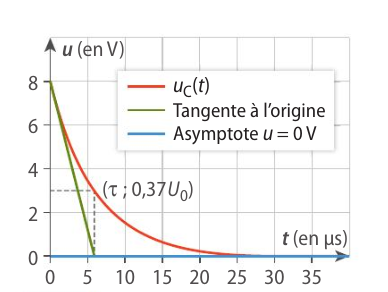
\includegraphics[scale=0.65]{figures/rc/tau_decharge}	
\end{center}


\textbf{Première méthode }:\\
Calculons $u_c(\tau)$ : $u_c(\tau)=Ee^{-\tau/\tau}=\trou{0,37}\times E$\\
Afin de déterminer $\tau$, il suffit donc de tracer la droite d'équation $u=0,37.E$ et de lire l'abscisse du point d'intersection de cette droite avec la courbe représentant $u_c$ pendant la décharge.\\
\textbf{Deuxième méthode : }\\
On trace la tangente à l'origine. Cette tangente coupe l'axe \trou{des abscisses}  à la date t=$\tau$.




		\subsection{Etude de la charge}
 	
 	\blocgris{Situation}{
 
Un condensateur est monté en série avec un dipôle ohmique de résistance R et une source de tension E.
L'interrupteur est initialement ouvert, on le ferme au temps t=0s.\\
On étudie les variations de la tension $u_c$ au cours du temps.
\\
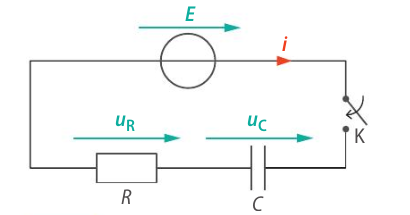
\includegraphics[scale=0.5]{figures/rc/circuit_charge}
}

\etiquetterouge{Objectif} Trouver l'expression mathématique de la tension $u_c(t)$ aux bornes du condensateur pendant sa charge.\\


\etiquette{Etape 1}
D'après la loi des mailles dans le circuit, on a :
\begin{center}
$\trou{E}=u_c+u_R$ 
\end{center}
\etiquette{Etape 2}
$$u_R=Ri=\trou{RC\dfrac{du_c}{dt}}$$
On en déduit que :
\begin{center}
$RC . \trou{\dfrac{du_c}{dt}}+\trou{u_c}=E$\\
\end{center}

et donc en divisant tous les termes par $RC$ 
$$\dfrac{du_c}{dt}+\dfrac{1}{RC}.u_c=\dfrac{E}{RC}$$
On ordonne les termes afin d'obtenir la forme $y' = ay + b$
$$\boxed{\dfrac{du_c}{dt}=-\dfrac{1}{RC}.u_c+\dfrac{E}{RC}}$$
Comme pour la décharge, il s'agit d'une équation différentielle du premier ordre. Résoudre cette équation c'est trouver la fonction $u_c(t)$.

\etiquette{Résolution de l'équation différentielle}

On cherche $u_c(t)$ telle que $$\boxed{\dfrac{du_c}{dt}=-\dfrac{1}{RC}.u_c+\dfrac{E}{RC}}$$ avec $$u_c(t=0)= 0\:V \quad\text{condition initiale}$$

Utilisons l'outil mathématique avec: $a=\trou{-1/RC}$, $b=\trou{\frac{E}{RC}}$ soit $-\frac{b}{a}=E$ (à vérifier vous même!!)\\
Cette équation a une solution de la forme $u_c(t)=\trou{K e^{-t/RC}+E}$\\
Déterminons K, en utilisant $$u_c(0)=0\quad\text{et aussi}\quad u_c(0)=Ke^0+E$$ donc $$K=\trou{-E}\quad\Rightarrow u_c(t)=\trou{-E.e^{-t/RC}} + \trou{E}$$ En factorisant par E: $$\boxed{u_c(t)=E\times \left( 1- e^{-t/RC}\right)}$$
	 
\etiquette{Représentation graphique de $u_c(t)$}\\
\begin{center}
	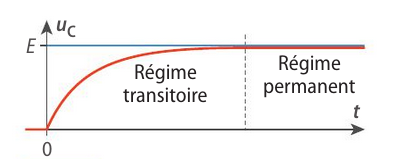
\includegraphics[width=0.4\textwidth]{figures/rc/courbe_charge}	
	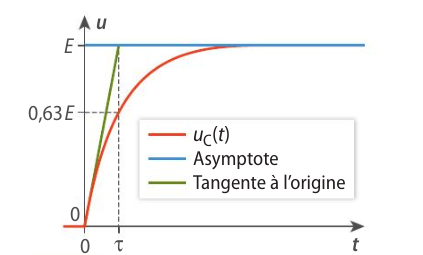
\includegraphics[width=0.6\textwidth]{figures/rc/tau}
\end{center}

\paragraph*{Observations} 
\begin{itemize}
	\item On constate qu'après une certaine durée, la tension du condensateur n'évolue plus. On dit que le régime \trou{transitoire} est terminé et que le régime \trou{permanent} est atteint.  
	\item Après $5\times \tau$ l'écart entre $u_c(t)$ et son asymptote est de moins de 1 \%.
\end{itemize}

\etiquette{Détermination de $\tau$}
\textbf{Première méthode }:\\
Calculons $u_c(\tau)$ : $u_c(\tau)=E(1-e^{-\tau/\tau})=E(1-e^{-1})=0,63E$\\
Afin de déterminer $\tau$, il suffit donc de tracer la droite d'équation $u=0,63E$ et de lire l'abscisse du point d'intersection de cette droite avec la courbe représentant $u_c$ pendant la charge.\\
\textbf{Deuxième méthode : }\\
On trace la tangente à l'origine. Cette tangente coupe l'asymptote $u_c=E$ à la date t=$\tau$.

	 
	\section*{Exercices à faire}
A partir de la page \textbf{434} et suivantes \\
\begin{itemize}
	\item Restituer le cours: 3, 4, 10, 11	 
	\item Etablir l'équation différentielle: 12, 13
	\item Résoudre l'équation différentielle: 15, 16
	\item Mesure de $\tau$: 18
	\item Synthèse: Lire les bons réflexes p 434 - Faire et étudier en détail l'ex1 p 434 
	\item S'entraîner pour le contrôle 19, 21
	\item Préparer le BAC: 30	 
	

\end{itemize}

Un sujet de bac: Amérique du nord 2021 Sujet 1 Exercice 1 Partie B

 \url{https://labolycee.org/un-sport-traditionnel-le-lancer-de-gerbe-de-paille}
	 
	 